\documentclass[11pt,a4paper]{ctexart}

% ============ 版面与宏包 ============
\usepackage[a4paper,top=1.9cm,bottom=1.7cm,left=1.75cm,right=1.75cm]{geometry}
\usepackage{graphicx}
\usepackage{booktabs}
\usepackage{tabularx}
\usepackage{array}
\usepackage{longtable}
\usepackage{xcolor}
\usepackage{enumitem}
\usepackage{listings}
\usepackage{caption}
\usepackage{titlesec}
\usepackage{fancyhdr}
\usepackage{tcolorbox}
\usepackage{tikz}
\usetikzlibrary{arrows.meta,positioning,shapes.geometric,fit,backgrounds,calc}
\usepackage[hidelinks]{hyperref}
\setcounter{tocdepth}{1}

\definecolor{teal}{HTML}{0F766E}
\definecolor{lightteal}{HTML}{E3F3F0}
\definecolor{sand}{HTML}{FAFAF8}
\definecolor{linegrey}{HTML}{D8DAD3}
\definecolor{ink}{HTML}{1B1D1A}
\definecolor{muted}{HTML}{6C7168}
\definecolor{warm}{HTML}{B45309}
\definecolor{warmsoft}{HTML}{FDF1E0}

\captionsetup{font=small,labelfont={bf,color=teal},justification=centering,skip=4pt}
\titleformat{\section}{\normalfont\large\bfseries\color{teal}}{\thesection}{0.6em}{}
\titleformat{\subsection}{\normalfont\normalsize\bfseries}{\thesubsection}{0.5em}{}
\titleformat{\subsubsection}{\normalfont\normalsize\bfseries\color{muted}}{\thesubsubsection}{0.5em}{}
\titlespacing*{\section}{0pt}{10pt}{5pt}
\titlespacing*{\subsection}{0pt}{7pt}{3pt}
\titlespacing*{\subsubsection}{0pt}{6pt}{2pt}
\setlist[itemize]{leftmargin=1.4em,itemsep=1pt,topsep=2pt,parsep=0pt}
\setlist[enumerate]{leftmargin=1.7em,itemsep=1pt,topsep=2pt,parsep=0pt}
\linespread{1.06}
\setlength{\parskip}{1pt}

\pagestyle{fancy}
\setlength{\headheight}{22pt}
\fancyhf{}
\fancyhead[L]{\footnotesize\color{muted}溯理成画 · AI 定理讲解视频生成系统}
\fancyhead[R]{\footnotesize\color{muted}iCAN 挑战赛道 · AI 应用创新挑战赛}
\fancyfoot[C]{\footnotesize\thepage}
\renewcommand{\headrulewidth}{0.3pt}
\renewcommand{\headrule}{\hbox to\headwidth{\color{linegrey}\leaders\hrule height \headrulewidth\hfill}}

\ctexset{
  section/format = \raggedright,
  subsection/format = \raggedright,
}

\lstset{
  basicstyle=\ttfamily\footnotesize,
  breaklines=true,
  breakatwhitespace=false,
  frame=single,
  framesep=4pt,
  rulecolor=\color{linegrey},
  backgroundcolor=\color{sand},
  columns=fullflexible,
  keepspaces=true,
  showstringspaces=false,
  xleftmargin=4pt,
  xrightmargin=4pt,
  aboveskip=6pt,
  belowskip=6pt,
}

\newtcolorbox{keybox}[1][]{
  colback=lightteal, colframe=teal, boxrule=0.4pt, arc=2pt,
  left=6pt, right=6pt, top=5pt, bottom=5pt, #1
}
\newtcolorbox{notebox}[1][]{
  colback=warmsoft, colframe=warm, boxrule=0.4pt, arc=2pt,
  left=6pt, right=6pt, top=5pt, bottom=5pt, #1
}

\tikzset{
  layerbox/.style={draw=linegrey, fill=sand, rounded corners=2pt, align=center,
    inner sep=4pt, minimum height=0.8cm, font=\scriptsize},
  accentbox/.style={draw=teal, fill=lightteal, rounded corners=2pt, align=center,
    inner sep=4pt, minimum height=0.8cm, font=\scriptsize},
  enginebox/.style={draw=teal, fill=white, rounded corners=2pt, align=center,
    inner sep=4pt, minimum height=0.8cm, font=\scriptsize},
  flow/.style={-{Latex[length=2mm]}, draw=muted, line width=0.5pt},
  backflow/.style={-{Latex[length=2mm]}, draw=warm, line width=0.5pt, dashed},
  layerlabel/.style={font=\scriptsize\bfseries, color=muted, anchor=north west},
}

\begin{document}
\sloppy
\setlength{\emergencystretch}{2em}

% ==================== 封面 ====================
\thispagestyle{empty}
\begin{center}
\vspace*{2.4cm}

\includegraphics[width=3.2cm]{logo.png}\\[0.5cm]
{\Huge\bfseries\color{teal} 溯理成画}\\[0.25cm]
{\Large AI 定理讲解视频生成系统}\\[0.35cm]
{\large\color{muted} 把一个定理，自动变成一段带讲解的动画视频}\\[1.1cm]

\rule{\textwidth}{0.4pt}\\[0.35cm]
{\large\bfseries 参赛作品文档}\\[0.2cm]
{\normalsize iCAN 国际大学生创新创业大赛 · 挑战赛道「AI 应用创新挑战赛」}\\[0.35cm]
\rule{\textwidth}{0.4pt}\\[1.1cm]

\begin{minipage}{0.86\textwidth}
\begin{tcolorbox}[colback=sand,colframe=linegrey,boxrule=0.4pt,arc=2pt,
  left=10pt,right=10pt,top=8pt,bottom=8pt]
\centering\small
\textbf{作品一句话定位}\\[3pt]
基于开源学术项目 TheoremExplainAgent（ACL 2025 主会 Oral）完成\textbf{中文化改造与产品化落地}：
把一个「只能生成英文、只能命令行操作、成功率不稳定」的科研原型，
做成面向中文用户、旁白／字幕／画面全中文、可在本地一键使用的定理讲解视频生成系统。
\end{tcolorbox}
\end{minipage}\\[1.0cm]

\begin{tabular}{@{}r@{\quad}l@{}}
\small\color{muted} 作品名称： & \small 溯理成画 —— AI 定理讲解视频生成系统 \\
\small\color{muted} 作品形态： & \small 本地 Web 应用（FastAPI）+ 多智能体视频生成流水线 \\
\small\color{muted} 核心技术： & \small 大模型分镜与代码生成 · 自动纠错闭环 · LaTeX-CJK 中文画面渲染 · 神经语音合成 \\
\small\color{muted} 生成引擎来源： & \small 开源项目 TheoremExplainAgent（MIT 协议，已如实标注出处） \\
\small\color{muted} 完成日期： & \small 2026 年 9 月 \\
\end{tabular}
\end{center}

\clearpage

% ==================== 目录 ====================
{\small
\renewcommand{\contentsname}{\color{teal}目\quad 录}
\tableofcontents
}
\clearpage

% ==================== 1 作品概述 ====================
\section{作品概述}

\subsection{一句话说明}

\textbf{一句话定位：}输入一个定理名称和一句背景说明，系统自动完成「教学法规划 → 分镜脚本 → 视觉设计 → Manim 动画代码生成 → 渲染纠错 → 中文配音 → 字幕与成片合成」的全流程，产出可直接用于教学的讲解视频。

\textbf{一句话差异化：}同类科研原型只解决「能不能生成」，我们解决「中文能不能用、普通人能不能用、失败之后能不能救回来」。

\subsection{作品形态与交付物}

本作品交付的是一个\textbf{可在本机一键启动的 Web 应用}与\textbf{一套完整的多智能体生成流水线}，具体包括：

\begin{itemize}
  \item \textbf{可视化操作界面}：任务创建、参数配置、环境自检、实时进度、分幕回放、成片播放与下载，全程图形化操作，无需命令行；
  \item \textbf{中文生成能力}：中文旁白、中文字幕、画面中的中文标题与标签（纯数学公式保持标准 LaTeX）；
  \item \textbf{稳定性与容错机制}：常见错误提示词注入、错误日志聚焦裁剪、自动修复重试、分幕跳过与「部分成功」兜底成片；
  \item \textbf{可复现的工程结构}：任务队列、日志持久化、产物目录规范、评测脚本与示例题库。
\end{itemize}

\subsection{与开源基线的关系（诚实出处声明）}

本作品的核心生成引擎来自开源项目 \textbf{TheoremExplainAgent}（论文 \textit{TheoremExplainAgent: Towards Video-based Multimodal Explanations for LLM Theorem Understanding}，\textbf{ACL 2025 主会 Oral}，TIGER-AI-Lab 团队，arXiv:2502.19400，MIT 协议并附 research-only 声明）。

我们\textbf{不声称}发明了「定理讲解视频生成」这一算法。本作品的贡献是在其之上所作的中文化与产品化\textbf{工程增量}，边界如下表所示。

\begin{table}[htbp]
\centering
\small
\caption{上游能力与本作品增量对照}
\begin{tabularx}{\textwidth}{@{}p{2.5cm} p{4.9cm} X@{}}
\toprule
\textbf{维度} & \textbf{上游 TheoremExplainAgent} & \textbf{本作品（溯理成画）} \\
\midrule
交互方式 & 命令行传参，需要配置 PYTHONPATH、模型、输出目录 & 浏览器一键操作，任务队列、进度与日志可视化 \\
讲解语言 & 仅英文旁白；画面上刻意全部使用英文以避免中文渲染失败 & 中文旁白（免费神经语音）、中文字幕，\textbf{画面标题／标签亦可显示中文} \\
中文排版 & 默认 \texttt{latex} 引擎无法排版 CJK，画面不允许出现中文 & 切换到 \texttt{xelatex + ctex} 全局模板，公式仍为标准 LaTeX \\
成功率 & 模型写错 Manim API 时反复失败，缺少针对性提示 & 注入常见错误速查表 + 错误日志聚焦裁剪，提高一次通过率与修复成功率 \\
失败后果 & 任一幕失败即无成片 & 逐幕状态可视、可只重跑失败分幕；有成片兜底（部分分幕版本） \\
工程缺陷 & 视觉修复分支引用未赋值变量，触发即崩溃；ffmpeg 管道死锁风险 & 已修复上述缺陷 \\
\bottomrule
\end{tabularx}
\end{table}

\begin{keybox}
\textbf{为什么要把「出处」写在最前面：}本作品是工程落地与产品化创新，不是算法原创。如实标注上游、清晰界定增量，既是对开源作者著作权的尊重，也是技术评审中最经得起追问的表达方式。
\end{keybox}

% ==================== 2 项目背景 ====================
\section{项目背景}

\subsection{宏观背景：教育数字化与「AI + 教育」的确定性趋势}

教育内容的生产方式正在被大模型重构。过去，一节高质量的可视化教学视频依赖「学科专家 + 脚本 + 动画师 + 配音 + 剪辑」的多人协作，周期以周计；而大模型已经具备把\textbf{自然语言意图}翻译为\textbf{可执行可视化代码}的能力，使「用一句话生成一段教学动画」在技术上第一次成为可能。

与此同时，国家层面对教育数字化持续加码，《教育强国建设规划纲要》《人工智能+教育》等政策方向均明确鼓励智能技术进入教学场景；各级学校普遍开展微课、翻转课堂与数字化备课，对\textbf{可自主生产、可反复修改、成本可控}的教学视频有持续而真实的需求。

\subsection{技术背景：定理讲解视频生成的学术前沿}

2025 年，TIGER-AI-Lab 提出 TheoremExplainAgent 并发表于 ACL 2025 主会（Oral，Top 3\%）。该工作第一次系统性地证明：让大模型生成\textbf{长时段 Manim 动画}，可以形成对定理的「视频式多模态解释」，并且这种解释方式能够暴露出纯文本推理中容易被隐藏的逻辑漏洞。

这套引擎证明了两件事：

\begin{enumerate}
  \item \textbf{方向成立}——「代码即动画」的路线足以承载严谨的数学讲解；
  \item \textbf{产品不成立}——它是一份科研代码：只有英文、只有命令行、对模型能力高度敏感、失败即无产出。
\end{enumerate}

换言之，学术侧解决了 0 到 1 的可行性，产业侧 1 到 100 的可用性仍然空白。这个空白，正是本作品选择的切入点。

\subsection{市场背景：中文教育内容生产的结构性缺口}

中文理科教学中，「抽象概念讲不清」是最顽固的痛点之一。函数变换、向量运算、概率分布、微积分基本定理这类内容，用板书或静态 PPT 讲解时，学习者往往「看得懂每一步、串不起来整条逻辑」。动态可视化本可显著改善理解，但中文世界缺少一条「低成本、可批量、面向教师个人」的生产线：

\begin{itemize}
  \item 国外成熟的动画工具（Manim 等）学习曲线陡峭，教师个人几乎不可能掌握编程式动画；
  \item 现成的通用 AI 视频工具擅长「讲解口播 + 素材拼接」，却\textbf{无法保证数学正确性}，更无法生成精确的坐标轴、函数图像与公式推导动画；
  \item 现有开源方案几乎全部以英文为中心设计，中文化不是「换个语音」那么简单（详见第 7.3 节）。
\end{itemize}

% ==================== 3 痛点分析 ====================
\section{痛点问题分析}

\subsection{学习者侧：抽象知识的「理解断层」}

\begin{itemize}
  \item \textbf{静态媒介承载不了动态过程}：板书与 PPT 只能展示「结果」，而数学理解依赖「过程」——变换、逼近、构造、推导；
  \item \textbf{缺少分层讲解}：同一知识点，初学者需要从几何直觉切入，进阶者需要严格证明，现有资源很难同时满足；
  \item \textbf{注意力与节奏不可控}：长视频无法按需跳转到「我卡住的那一步」，理解断点难以定位。
\end{itemize}

\subsection{教师与创作者侧：制作成本高、门槛高、周期长}

\begin{itemize}
  \item \textbf{人力成本}：一段 8 分钟的高质量数学动画，传统流程需要学科专家 + 动画师协作，制作周期通常以周计；
  \item \textbf{技术门槛}：Manim 属于「编程式动画框架」，需要同时掌握 Python、LaTeX 与空间布局，普通教师难以跨过；
  \item \textbf{不可复用}：一次制作的动画与具体题目强绑定，换一个例题几乎要从头再来；
  \item \textbf{无法本地化}：即便使用国外工具，也难以生成符合中文教学表达习惯的讲解稿与字幕。
\end{itemize}

\subsection{工具侧：现有方案的四类具体缺陷}

我们在实际跑通开源引擎的过程中，把缺陷定位到了非常具体的位置，这也是本作品全部工程工作的问题来源：

\begin{enumerate}
  \item \textbf{语言缺陷}：仅支持英文旁白；画面文本强制英文——因为默认 LaTeX 引擎无法排版中文，中文会直接导致渲染失败；
  \item \textbf{稳定性缺陷}：模型极易写出已被废弃或写错的 Manim API（如 \texttt{ShowCreation}、\texttt{get\_graph}、\texttt{x\_range} 参数形式等），一次失败即浪费数分钟渲染时间；
  \item \textbf{可恢复性缺陷}：任一分幕失败则整部视频没有产出，用户既拿不到部分成果，也无从判断问题出在哪一幕；
  \item \textbf{可用性缺陷}：安装与运行依赖命令行、环境变量与路径配置，非技术用户无法独立完成。
\end{enumerate}

\subsection{痛点—需求—功能映射}

\begin{table}[htbp]
\centering
\small
\caption{从痛点到功能的正向追溯（保证「每个功能都在解决真实问题」）}
\begin{tabularx}{\textwidth}{@{}p{3.4cm} p{4.2cm} X@{}}
\toprule
\textbf{痛点} & \textbf{需求} & \textbf{对应功能} \\
\midrule
中文用户看不懂英文讲解 & 讲解内容全中文 & 中文旁白 + 中文字幕 + 语言一键切换 \\
画面停留在英文 & 画面标题／标签中文化 & xelatex + ctex 全局模板自动注入 \\
不懂编程、不会命令行 & 图形化完成全部操作 & Web 界面、示例题库、环境自检 \\
模型写错动画 API 导致失败 & 提高一次成功率 & 常见错误速查表注入、约束提示词 \\
失败后不知错在哪 & 可见、可诊断 & 实时日志、逐幕状态、API 错误人话提示 \\
一幕失败则全盘无产出 & 部分结果为可用成果 & 只重跑失败分幕、部分分幕兜底成片 \\
生成过程像黑盒 & 过程可观测 & 分幕进度、阶段命名、用时统计 \\
想先花几十秒验证链路 & 快速试跑通道 & 「只生成分镜脚本」模式 \\
\bottomrule
\end{tabularx}
\end{table}

% ==================== 4 需求分析 ====================
\section{需求分析}

\subsection{分析方法与依据}

本作品的需求并非凭空设想，而是通过三条相互印证的路径得出：

\begin{enumerate}
  \item \textbf{上游代码走查}：逐文件梳理生成流水线的阶段划分、模型调用点与失败模式，定位可工程化的改进位点；
  \item \textbf{真实运行观测}：在本机以真实模型多次跑通完整流程，记录每一幕的失败原因、重试次数与耗时，把「失败」当作需求的一等来源；
  \item \textbf{场景化推演}：围绕教师备课、学生自学、内容创作者批量生产三类典型场景，推演完整使用链路与断点。
\end{enumerate}

\subsection{功能需求}

\begin{table}[htbp]
\centering
\small
\caption{功能需求清单}
\begin{tabularx}{\textwidth}{@{}p{1.5cm} p{4.1cm} X@{}}
\toprule
\textbf{编号} & \textbf{需求名称} & \textbf{说明} \\
\midrule
FR1 & 任务创建 & 输入定理／主题、一句话背景，选择语言、模型、画质、重试次数后提交生成任务 \\
FR2 & 示例题库 & 内置勾股定理、贝叶斯定理、傅里叶级数等可直接运行的主题，一键填充表单 \\
FR3 & 环境自检 & 启动即检测 Python 环境、ffmpeg、中英文配音、各模型 Key 状态，异常项显式提示 \\
FR4 & 密钥管理 & 在界面内填写／更新模型 API Key，落盘至本地 \texttt{.env}，不写入代码仓库 \\
FR5 & 任务队列 & 串行调度渲染任务，避免多任务争抢 CPU 导致整体变慢 \\
FR6 & 实时进度 & 显示分幕总数、已完成数、当前阶段与已运行时长 \\
FR7 & 运行日志 & 完整输出运行日志，支持自动滚动，错误可直接定位到具体分幕 \\
FR8 & 错误人话提示 & 把「余额不足」「Key 无效」「触发限流」等 API 错误翻译为可执行的中文提示 \\
FR9 & 分幕回放 & 每一幕渲染成功后均可单独播放，便于检查单幕质量 \\
FR10 & 成片播放与下载 & 支持在线播放、下载视频与下载字幕文件 \\
FR11 & 部分成功兜底 & 有分幕失败时，自动把成功的分幕拼成可播放的「部分分幕」版本 \\
FR12 & 失败分幕重试 & 已完成的分幕直接复用，只重新生成失败分幕，避免重复消耗 \\
FR13 & 任务生命周期管理 & 支持取消运行中的任务、移除历史记录 \\
FR14 & 中英文切换 & 同一主题可在中文模式与英文模式之间任意切换，英文行为与上游一致 \\
FR15 & 快速试跑 & 「只生成分镜脚本」模式跳过渲染，几十秒至数分钟即可验证链路与中文旁白 \\
\bottomrule
\end{tabularx}
\end{table}

\subsection{非功能需求}

\begin{table}[htbp]
\centering
\small
\caption{非功能需求与设计对策}
\begin{tabularx}{\textwidth}{@{}p{2.6cm} p{4.6cm} X@{}}
\toprule
\textbf{类别} & \textbf{要求} & \textbf{设计对策} \\
\midrule
可用性 & 非技术用户可独立完成全流程 & 全图形化操作；默认值合理；错误提示给出下一步动作 \\
可观测性 & 长任务过程不黑盒 & 以产物文件（分镜大纲、逐幕计划、渲染成功标记）反推进度，进度天然可信 \\
健壮性 & 单点失败不导致整体不可用 & 逐幕隔离；失败重试；兜底合并；取消与重试接口 \\
性能 & 单机可跑、耗时可预期 & 提供三档画质；草稿档 480p15；任务串行避免互相拖慢 \\
兼容性 & 中文环境不崩溃 & 中文 TTS 或 CJK 模板缺失时静默降级为可用配置，而非直接报错 \\
安全与隐私 & 密钥不外泄、服务不暴露 & 仅监听 \texttt{127.0.0.1}，密钥存本地 \texttt{.env}，视频与日志不出本机 \\
可复现性 & 结果可复现、过程可回溯 & 每次生成独立目录；代码版本、修复日志、错误日志全部落盘 \\
可扩展性 & 可替换模型与语音引擎 & 模型经 LiteLLM 统一接入；语音服务以工厂函数按语言分发 \\
\bottomrule
\end{tabularx}
\end{table}

\subsection{需求优先级}

采用 MoSCoW 方法排序：\textbf{Must}（FR1、FR3、FR5--FR7、FR10、FR11、FR14）；\textbf{Should}（FR2、FR4、FR8、FR9、FR12、FR15）；\textbf{Could}（FR13 及画质档位细化、任务统计看板）；\textbf{Won't（本期）}：云端多租户、在线协作、视频在线编辑。

% ==================== 5 目标用户 ====================
\section{目标用户群体}

\subsection{用户画像}

\begin{table}[htbp]
\centering
\small
\caption{四类目标用户及其核心诉求}
\begin{tabularx}{\textwidth}{@{}p{2.5cm} p{3.3cm} p{4.2cm} X@{}}
\toprule
\textbf{用户群体} & \textbf{典型特征} & \textbf{核心诉求} & \textbf{关键使用场景} \\
\midrule
中学／大学学生 & 自学与复习，面对抽象概念容易卡壳 & 需要「看得见过程」的讲解，且要是中文 & 课后补弱、考研／竞赛复习、翻转课堂预习 \\
一线教师 & 备课时间紧，不掌握编程式动画 & 快速产出可讲解的动画素材，能按自己的讲法调整 & 新课导入、难点突破、公开课与微课制作 \\
教育内容创作者／机构 & 需要批量、稳定、可定制的内容产能 & 批量生产、统一风格、可控成本 & 知识类短视频、题库配套讲解、课程配套动画 \\
企业培训／科普 & 需要把抽象原理讲给非专业人群 & 用最少的制作成本讲清概念 & 技术培训、产品原理演示、科普内容 \\
\bottomrule
\end{tabularx}
\end{table}

\subsection{典型使用场景}

\textbf{场景一（学生自学）}：复习到「傅里叶级数」时无法理解「用正弦波叠加逼近方波」，输入该主题并生成一段中文讲解视频，重点观看分幕中的「逐项叠加」动画，配合字幕反复理解。

\textbf{场景二（教师备课）}：需要在课堂上讲清「贝叶斯定理中先验的更新过程」，用系统生成草稿视频，检查旁白与画面是否符合自己的讲解思路，再据此调整课堂讲解顺序，把成片作为课堂素材。

\textbf{场景三（创作者批量生产）}：围绕一个知识主题清单（如「微积分基本定理」「欧拉公式」）批量生成初稿视频，人工筛选后再做二次加工，把单条内容的制作成本与周期压到最低。

\subsection{市场规模量级（估算）}

仅以国内教育从业者与高教／中学理科学习者计，潜在用户规模在\textbf{千万级}；其中愿意为「内容生产效率」直接付费的教师与内容创作者，量级在\textbf{百万级}。本作品的市场空间不依赖「替代现有教育平台」，而依赖「把原本因成本过高而不存在的教学动画，变成可被批量生产的内容」。

% ==================== 6 开发工具 ====================
\section{开发工具与技术栈}

\subsection{工具与技术清单}

\begin{table}[htbp]
\centering
\small
\caption{开发工具与技术栈及其在本作品中的职责}
\begin{tabularx}{\textwidth}{@{}p{2.7cm} p{3.5cm} X@{}}
\toprule
\textbf{类别} & \textbf{工具／技术} & \textbf{在本作品中的职责} \\
\midrule
语言与运行时 & Python 3.12 & 生成流水线、服务端、工具脚本的统一语言 \\
Web 服务 & FastAPI + Uvicorn & 提供 REST 接口、静态页面托管、任务提交与查询 \\
任务调度 & threading + queue + subprocess & 串行任务队列；以子进程隔离每次生成，避免模型调用与渲染互相污染 \\
前端 & 原生 HTML + CSS + JavaScript & 零构建步骤的界面，开箱即用，无前端工具链依赖 \\
大模型接入 & LiteLLM & 用统一的模型命名与调用方式接入 DeepSeek、OpenAI、Gemini 等模型 \\
动画引擎 & Manim Community 0.18 & 执行「代码即动画」，精确绘制坐标轴、函数图像与几何构造 \\
语音同步 & manim-voiceover & 把旁白音频与动画时间轴绑定，自动生成字幕时间码 \\
语音合成 & edge-tts（中文）／ Kokoro（英文） & 免费中文神经语音／本地英文语音，无需付费接口即中文可用 \\
公式排版 & LaTeX + xelatex + ctex（MiKTeX 发行版） & 渲染数学公式；中文模式下提供 CJK 排版能力 \\
视频处理 & FFmpeg / ffprobe（随仓库分发） & 统一编码参数、拼接分幕、生成可流式播放的成片 \\
质量评测 & eval\_suite + TheoremExplainBench 数据 & 对成片做文本／图像／视频维度的自动评估 \\
工程协作 & Git（保留上游 LICENSE 与提交历史） & 版本管理与出处可追溯 \\
渲染验证 & 无头浏览器（Edge headless） & 页面与配图的自动化截图与核验 \\
\bottomrule
\end{tabularx}
\end{table}

\subsection{选型理由}

\begin{itemize}
  \item \textbf{选择 Manim 而不是通用视频生成模型}：通用文生视频模型擅长的画面质感，恰恰是数学讲解最不需要的；数学讲解需要的是\textbf{精确、可复现、可推导}的图形与公式。Manim 用确定性代码换取数学正确性，这是本场景唯一可接受的技术路线。
  \item \textbf{选择 LiteLLM 而不是直接绑定某一家模型}：教育场景对成本敏感，且不同模型写 Manim 代码的能力差异很大。统一接入层让使用者可以按预算与效果自由更换模型，也避免了被单一供应商锁定。
  \item \textbf{选择 edge-tts 作为中文语音}：免费、无需 API Key、音质达到教学可用水平，且支持中文神经语音与语速控制，显著降低了中文用户的上手门槛；英文侧保留上游 Kokoro 本地引擎，保证零回归。
  \item \textbf{选择 FastAPI + 原生前端}：任务生成本质是「长耗时后台作业 + 前端轮询」。FastAPI 的异步与静态托管能力足够，再叠加原生前端即可实现零构建部署，避免为界面引入不必要的工程复杂度。
\end{itemize}

% ==================== 7 技术方案 ====================
\section{实现作品的技术方案}

\subsection{总体架构}

系统采用\textbf{「Web 服务层 + 生成流水线层 + 能力层」}的三层结构：Web 服务层负责交互与调度，生成流水线层负责「把主题变成视频」，能力层由大模型、语音合成、LaTeX 排版与渲染工具构成。

\begin{figure}[htbp]
\centering
\begin{tikzpicture}[scale=0.96]
  % 交互层
  \node[accentbox, text width=11.6cm] (ui) at (0,0)
    {\textbf{浏览器交互层}：新建任务 · 参数配置（语言／模型／画质）· 环境自检 · 实时进度 · 日志 · 分幕回放 · 成片播放与下载};
  % 服务层
  \node[layerbox, text width=11.6cm] (svc) at (0,-1.30)
    {\textbf{服务层（本作品自研）}：FastAPI 接口 · 串行任务队列 · 进度解析 · 日志流 · \texttt{.env} 密钥管理 · 静态前端};
  % 执行层
  \node[layerbox, text width=11.6cm] (run) at (0,-2.60)
    {\textbf{执行层}：子进程调用生成脚本，注入环境变量（讲解语言 / 渲染画质 / 编码设置）};
  % 引擎层
  \node[enginebox, text width=3.7cm] (planner) at (-4.30,-4.05) {\textbf{VideoPlanner}\\教学法框架 · 分镜大纲 · 逐幕细化计划};
  \node[enginebox, text width=3.7cm] (coder)   at (0.00,-4.05)  {\textbf{CodeGenerator}\\Manim 代码生成 · 自动修复};
  \node[enginebox, text width=3.7cm] (render)  at (4.30,-4.05)  {\textbf{VideoRenderer}\\渲染 · 配音 · 字幕 · 合成};
  % 能力层
  \node[layerbox, text width=2.6cm] (llm) at (-4.30,-5.65) {大模型（LiteLLM）\\DeepSeek／OpenAI／Gemini};
  \node[layerbox, text width=2.6cm] (tts) at (-1.45,-5.65) {语音合成\\edge-tts／Kokoro};
  \node[layerbox, text width=2.6cm] (tex) at (1.45,-5.65)  {LaTeX 排版\\xelatex + ctex};
  \node[layerbox, text width=2.6cm] (man) at (4.30,-5.65)  {Manim 渲染\\FFmpeg 合成};

  \draw[flow] (ui) -- (svc);
  \draw[flow] (svc) -- (run);
  \draw[flow] (run.south) -- ++(0,-0.30) coordinate (bus);
  \draw[muted, line width=0.5pt] ([xshift=3.0cm]bus) -- ([xshift=-3.0cm]bus);
  \draw[flow] ([xshift=-4.30cm]bus) -- (planner.north);
  \draw[flow] (bus) -- (coder.north);
  \draw[flow] ([xshift=4.30cm]bus) -- (render.north);
  \draw[flow] (planner.south) -- ++(0,-0.25) coordinate (bus2);
  \draw[muted, line width=0.5pt] ([xshift=3.0cm]bus2) -- ([xshift=-3.0cm]bus2);
  \draw[flow] ([xshift=-4.30cm]bus2) -- (llm.north);
  \draw[flow] ([xshift=-1.45cm]bus2) -- (tts.north);
  \draw[flow] ([xshift=1.45cm]bus2) -- (tex.north);
  \draw[flow] ([xshift=4.30cm]bus2) -- (man.north);

  \node[layerlabel] at (5.95,-0.62) {交互／自研};
  \node[layerlabel, color=teal] at (5.95,-2.62) {上游引擎 + 中文化改造};
  \node[layerlabel] at (5.95,-5.65) {能力层};
\end{tikzpicture}
\caption{系统总体架构：交互层、服务层、执行层、引擎层与能力层}
\end{figure}

\subsection{生成流水线}

一次完整生成由若干阶段串联而成，每个阶段都有明确的输入、产物与模型调用点。流水线的关键设计是\textbf{逐幕解耦}：每一幕独立生成代码、独立渲染、独立失败，因此可以单独重试、单独回放。

\begin{figure}[htbp]
\centering
\begin{tikzpicture}[scale=1, node distance=0pt]
  \node[enginebox, text width=6.0cm] (p1) at (0,0)      {\textbf{阶段 1 · 教学法规划}\\依据教学框架设计学习目标与内容结构};
  \node[enginebox, text width=6.0cm] (p2) at (0,-1.05)  {\textbf{阶段 2 · 分镜大纲}\\拆解为若干幕（如 7 幕），定义每幕目标与版式};
  \node[enginebox, text width=6.0cm] (p3) at (0,-2.10)  {\textbf{阶段 3 · 逐幕细化}\\视觉故事板 · 技术实现方案 · 动画与旁白脚本};
  \node[enginebox, text width=6.0cm] (p4) at (0,-3.15)  {\textbf{阶段 4 · 代码生成}\\产出 Manim 场景代码（注入约束与常见错误速查表）};
  \node[enginebox, text width=6.0cm] (p5) at (0,-4.20)  {\textbf{阶段 5 · 渲染与配音}\\Manim 渲染画面 + 神经语音合成 + 生成字幕时间码};
  \node[accentbox, text width=6.0cm] (p6) at (0,-5.25)  {\textbf{阶段 6 · 合成成片}\\拼接分幕、重排 CJK 字幕、输出可播放视频与字幕文件};

  \draw[flow] (p1) -- (p2);
  \draw[flow] (p2) -- (p3);
  \draw[flow] (p3) -- (p4);
  \draw[flow] (p4) -- (p5);
  \draw[flow] (p5) -- (p6);

  % 失败分支
  \node[layerbox, text width=3.6cm, fill=warmsoft, draw=warm] (fix) at (5.5,-3.90)
    {\textbf{自动修复闭环}\\裁剪错误日志 → 定位异常 → 重新生成代码};
  \draw[backflow] (p5.east) -- ++(0.35,0) |- (fix.east);
  \draw[backflow] (fix.north) -- ++(0,0.55) -| (p4.east);
  \node[font=\scriptsize, color=warm, anchor=south] at (3.4,-4.02) {渲染失败};
  \node[font=\scriptsize, color=warm, anchor=west] at (5.75,-4.55) {重试 $\leq$ 设定次数};
\end{tikzpicture}
\caption{生成流水线：六个阶段，以及渲染失败的自动修复闭环}
\end{figure}

\subsection{关键技术攻关}

\subsubsection{攻关一：LaTeX-CJK 中文画面渲染（核心技术贡献）}

上游方案刻意让画面上的标题、标签全部保持英文，原因很直接：Manim 默认使用 \texttt{latex} 引擎，该引擎无法排版中日韩字符，一旦模型在画面里写了中文，渲染就会直接失败。

我们的做法是：在中文模式下，把 Manim 的\textbf{全局 Tex 模板}切换为支持 CJK 的 \texttt{TexTemplateLibrary.ctex}（\texttt{xelatex + ctex}），并让它作为模块导入的副作用\textbf{自动生效}：

\begin{itemize}
  \item 生成的场景代码只需按约定导入语音服务模块，无需改动、也无需「记住」要设置模板；
  \item 提示词中同时告知模型：中文模式下画面允许中文，但\textbf{公式仍写成标准 LaTeX}，并且禁止用空模板覆盖已配置的 CJK 模板；
  \item 若运行环境缺少 xelatex／ctex，则\textbf{静默降级}为英文画面，保证「能出片」优先于「更好看」。
\end{itemize}

该能力已经过实际渲染验证（见第 11.3 节）：中文模式下生成的 LaTeX 源文件中出现了 \texttt{ctex} 宏包与中文 \texttt{\textbackslash text\{\}} 内容，并成功编译出矢量图形。

\subsubsection{攻关二：可插拔的中文语音引擎}

我们新增中文语音服务并以\textbf{工厂函数}统一分发：生成的代码只调用 \texttt{get\_speech\_service()}，由该函数根据环境变量中的讲解语言决定返回中文引擎（edge-tts）还是英文引擎（Kokoro）。这样带来三个好处：

\begin{enumerate}
  \item \textbf{同一份生成代码同时支持中英文}，语言切换不需要重新训练提示词或改代码；
  \item 英文模式行为与上游\textbf{完全一致}，未设置语言变量时零回归；
  \item 中文引擎不可用（离线或依赖缺失）时自动回退英文引擎，避免整条流程崩溃。
\end{enumerate}

\subsubsection{攻关三：提高代码一次通过率的「错误速查表」}

大模型（尤其是低成本模型）在编写 Manim 代码时高频踩同一批坑：使用已被移除的 \texttt{ShowCreation}、把 \texttt{axes.plot()} 写成 \texttt{get\_graph()}、坐标范围参数写成 \texttt{x\_min/x\_max}、在 \texttt{MathTex} 中忘记使用原始字符串等。

我们把这些错误整理为一份\textbf{「常见错误 → 正确写法」对照清单}，在「代码生成」与「错误修复」两个环节同时注入上下文，把模型从「试错」拉回「按规范写」。

\subsubsection{攻关四：错误日志聚焦与自动修复闭环}

Manim 的失败输出混杂了进度条、弃用警告与完整 traceback，直接塞给修复模型会把真正的异常淹没。我们新增日志裁剪：优先从最后一个 \texttt{Traceback} 位置截取，并对长度设上限、保留尾部关键信息。修复提示词中同时携带实现计划、原始代码与裁剪后的错误，使模型能够给出针对性修补而不是重写。

\subsubsection{攻关五：中文字幕重排与渲染管线修复}

\begin{itemize}
  \item \textbf{CJK 字幕重排}：上游按空格折行，中文几乎没有空格，导致整句字幕挤成一行。我们新增按标点与字数折行的后处理，仅在检测到 CJK 字符时生效，英文字幕保持原样；
  \item \textbf{修复上游缺陷}：视觉修复分支引用了从未赋值的模型变量，一旦触发即崩溃，已改为显式传参；
  \item \textbf{修复 ffmpeg 管道死锁}：合并视频时错误地接管了 stderr 却不读取，缓冲区写满即死锁，已改为让 stderr 正常继承；
  \item \textbf{渲染画质可配置}：把固定 1080p60 改为可配置档位，并提供草稿／推荐／高清三档，适配「快速试跑」与「正式出片」两种诉求。
\end{itemize}

\subsection{数据流与产物组织}

每次生成使用独立目录，保证过程可回溯：

\begin{lstlisting}
output/web/<topic>-<job_id>/<topic>/
  <topic>_scene_outline.txt          # 分镜大纲（SCENE_1..SCENE_n）
  scene1/ ... sceneN/
    code/<topic>_scene1_v0.py        # 每轮代码版本 v0, v1, v2 ...
    code/*_v1_error.log              # 该轮渲染错误
    subplans/*_vision_storyboard_plan.txt
    subplans/*_technical_implementation_plan.txt
    subplans/*_animation_narration_plan.txt
    succ_rendered.txt                # 该幕渲染成功标记
  media/videos/.../                 # 分幕视频与分幕字幕
  <topic>_combined.mp4 / .srt        # 官方合并成片与字幕
  <topic>_partial.mp4                # 部分分幕兜底成片
webapp/jobs/<job_id>.json / .log     # 任务元数据与完整运行日志
\end{lstlisting}

\subsection{质量评测体系}

仓库保留了上游的自动评测脚本与定理基准数据（TheoremExplainBench，240 条定理、覆盖数学／物理／计算机／化学四个学科、三档难度），可对成片做\textbf{文本、图像、视频}三个维度的模型化评估，用于后续迭代时「用数据决定改动是否真的更好」。评测体系不参与生成，只服务于验证与迭代。

% ==================== 8 AI 核心作用 ====================
\section{AI 功能在本作品中的核心作用}

\subsection{AI 不是外挂，而是作品本身}

本作品不是「先做一个视频工具，再顺手接一个大模型」，而是\textbf{把大模型当作系统的决策与生产能力本身}：从「教什么、怎么教」，到「画什么、怎么画」，再到「用什么声音讲」，全部由 AI 参与完成。整条流水线上有\textbf{七类 AI 环节}，每一环都是不可替换的：

\begin{table}[htbp]
\centering
\small
\caption{生成链路上的七类 AI 环节}
\begin{tabularx}{\textwidth}{@{}p{2.5cm} p{3.5cm} p{3.1cm} X@{}}
\toprule
\textbf{环节} & \textbf{输入 → 输出} & \textbf{使用的 AI 能力} & \textbf{若去掉该环节} \\
\midrule
A 教学法规划 & 主题 + 背景 → 学习目标与内容结构 & 大模型 + 教学设计提示词 & 视频退化为「公式罗列」，失去教学性 \\
B 分镜大纲 & 内容结构 → 若干幕的标题、目的、版式 & 大模型 + 结构化输出约束 & 无法拆分长视频，无法并行与容错 \\
C 逐幕细化 & 单幕目标 → 视觉故事板、技术实现、动画与旁白 & 大模型（多轮、可并行） & 动画没有镜头语言，画面与讲解脱节 \\
D 代码生成 & 细化计划 → 可执行的 Manim 场景代码 & 大模型代码生成 + 领域约束注入 & 系统无法产出任何画面 \\
E 自动修复 & 失败代码 + 聚焦错误 → 修正后的代码 & 大模型代码修复 & 一次失败即终止，成本不可控 \\
F 视觉自省 & 渲染视频／关键帧 → 视觉问题与修复建议 & 多模态大模型（VLM） & 画面重叠、出界、错位等「代码对但画面丑」的问题无法发现 \\
G 语音合成 & 旁白文本 → 带时间码的语音与字幕 & 神经语音合成 & 有画面无讲解，退化为静音动画 \\
\bottomrule
\end{tabularx}
\end{table}

\begin{keybox}
\textbf{核心判断：}在传统工具里，AI 是「可选项」——去掉它，工具仍然能用，只是慢一点。在本作品里，AI 是「唯一的生产力来源」——去掉任何一环，都得不到最终产物。这正是「AI 应用创新」的应有之义：不是给旧流程贴一个 AI 标签，而是用 AI 重建整个生产流程。
\end{keybox}

\subsection{环节 A｜教学法规划：把「讲一个定理」变成「设计一堂课」}

系统不会直接把主题丢给代码模型，而是先让大模型扮演\textbf{教学设计师}：明确学习目标（记忆／理解层、分析／评价层、应用／创造层）、规划内容结构（引入、背景、核心内容、练习、总结）并控制认知负荷。它同时约束了成片的节奏——例如引入部分只占全片时长的 5\%--10\%，核心内容占 60\%--70\%。

\textbf{这一环决定了作品的「教育质量下限」}：它保证输出不是一段「讲得挺热闹但没讲明白」的动画。

\subsection{环节 B｜分镜大纲：把长视频拆成可管理的幕}

大模型把内容结构展开为若干幕，每一幕都必须给出四项信息：\textbf{标题、教学目的（以及与上一幕的衔接）、画面内容描述、空间版式说明}（包含安全边距与元素最小间距）。并以结构化标签输出，便于程序稳定解析。

\textbf{这一环决定了作品的「工程可管理性」}：因为分成了独立的幕，才可能做到逐幕渲染、逐幕重试、逐幕回放与部分成功兜底。在本作品的实测中，一个 8 分钟量级的成片会被拆为 7 幕，单幕时长 27 秒至 131 秒不等。

\subsection{环节 C｜逐幕细化：把「一页脚本」变成「一套拍摄方案」}

对每一幕，系统并行地让模型产出三份彼此衔接的计划：\textbf{视觉故事板}（镜头里先出现什么、后出现什么、视线如何被引导）、\textbf{技术实现方案}（用哪些 Manim 对象与动画类）、\textbf{动画与旁白脚本}（每一段动画配哪一句讲解，并保持时间对齐）。这是「讲解语言」与「画面语言」对齐的关键环节，也是本作品把「AI 生成」升级为「AI 编排」的地方。

\subsection{环节 D｜代码生成：把方案翻译成精确的动画}

代码生成环节把细化计划翻译为可直接运行的 Manim 场景代码，并强制执行一组工程约束：必须继承语音同步场景类、必须通过工厂函数获取语音服务、必须显式导入全部所用对象、必须遵循安全边距与字号规范、必须使用当前版本仍然存在的 API。上下文里同时注入「Manim 速查表」「字号规范」「代码长度上限」「禁用写法清单」与我们新增的「常见错误速查表」。

\textbf{这是本作品最关键的一次「约束式 AI 应用」}：模型的创作自由度被放在「讲什么、怎么讲」上，而在「API 怎么写、版式怎么摆」上被强约束，从而在保留创造力的同时把失败率压下来。

\subsection{环节 E｜自动修复闭环：让 AI 自己把错误改对}

渲染失败时，系统不会立刻放弃，而是进入修复闭环：

\begin{enumerate}
  \item 捕获渲染进程的错误输出；
  \item \textbf{裁剪与聚焦}：从最后一个 traceback 处截取，剔除进度条与无关噪声；
  \item 把「实现计划 + 当前代码 + 聚焦后的错误 + 常见错误速查表」一并交给模型，要求产出完整可运行的新版本；
  \item 以新版本代码重新渲染，直到成功或达到设定的重试上限（默认 3 次，可配置 1--8 次）。
\end{enumerate}

整个过程留痕：每一轮代码都保存为独立版本（\texttt{v0, v1, v2 ...}），每轮错误单独落盘。用户既能看到「模型试了几次」，也能复盘「为什么失败」。

\subsection{环节 F｜视觉自省：用多模态模型检查「画面对不对」}

代码能跑通不等于画面讲得清。系统支持把渲染结果（对支持视频输入的模型直接送视频，其余模型送关键帧图像）交给多模态模型审阅，检查画面是否重叠、是否越界、是否与旁白错位，并给出修复建议。该能力把质量把关从「语法层」推进到「视觉层」，是自动化生成质量闭环的必要组成。

\subsection{环节 G｜语音合成与中文化：让讲解「说人话」}

每一句旁白由神经语音合成引擎生成音频，并与动画时间轴绑定，同时输出字幕时间码。中文模式下，系统通过环境变量向模型注入语言指令：\textbf{旁白必须使用中文}，画面标题与标签也可使用中文，而数学公式保持标准 LaTeX。配合第 7.3 节所述的 CJK 模板自动注入，最终实现「旁白、字幕、画面文字」三处一致的纯中文讲解。

\subsection{反证：如果没有 AI}

为了说明 AI 的核心作用，可以做一个简单的反向推演——把 AI 从系统中拿掉，剩下的是 Manim、FFmpeg 与 FFmpeg 之外的空白：

\begin{itemize}
  \item 没有大模型：没有人写得出这 7 幕的动画代码，除非雇佣动画工程师按周计价；
  \item 没有语音合成：视频是静音的，教学价值大幅下降；
  \item 没有多模态审阅：画面错误只能靠人一帧帧看；
  \item 没有修复闭环：一次 API 写错就要人工介入，成本不可预测。
\end{itemize}

结论很直接：\textbf{AI 是本作品的生产资料，而不是产品的装饰}。

\subsection{让 AI 可控：四条工程经验}

\begin{enumerate}
  \item \textbf{结构化输出优先}：要求模型以固定标签/字段输出，程序只解析结构，不猜测自然语言，杜绝「同一句话两种理解」带来的不稳定；
  \item \textbf{把领域知识做成清单注入}：高频错误与其正确写法以清单形式固定注入，比「请写正确的代码」有效得多；
  \item \textbf{把失败设计成流程的一部分}：预留重试、跳过、兜底与人工可见的日志，让「模型偶尔犯错」从事故变成常态；
  \item \textbf{把可替换性做进架构}：模型、语音引擎、画质档位都是可配置项，避免把产品绑死在某一家的能力与价格上。
\end{enumerate}

% ==================== 9 功能逐一说明 ====================
\section{作品功能逐一说明}

\subsection{界面总览}

\begin{figure}[htbp]
\centering
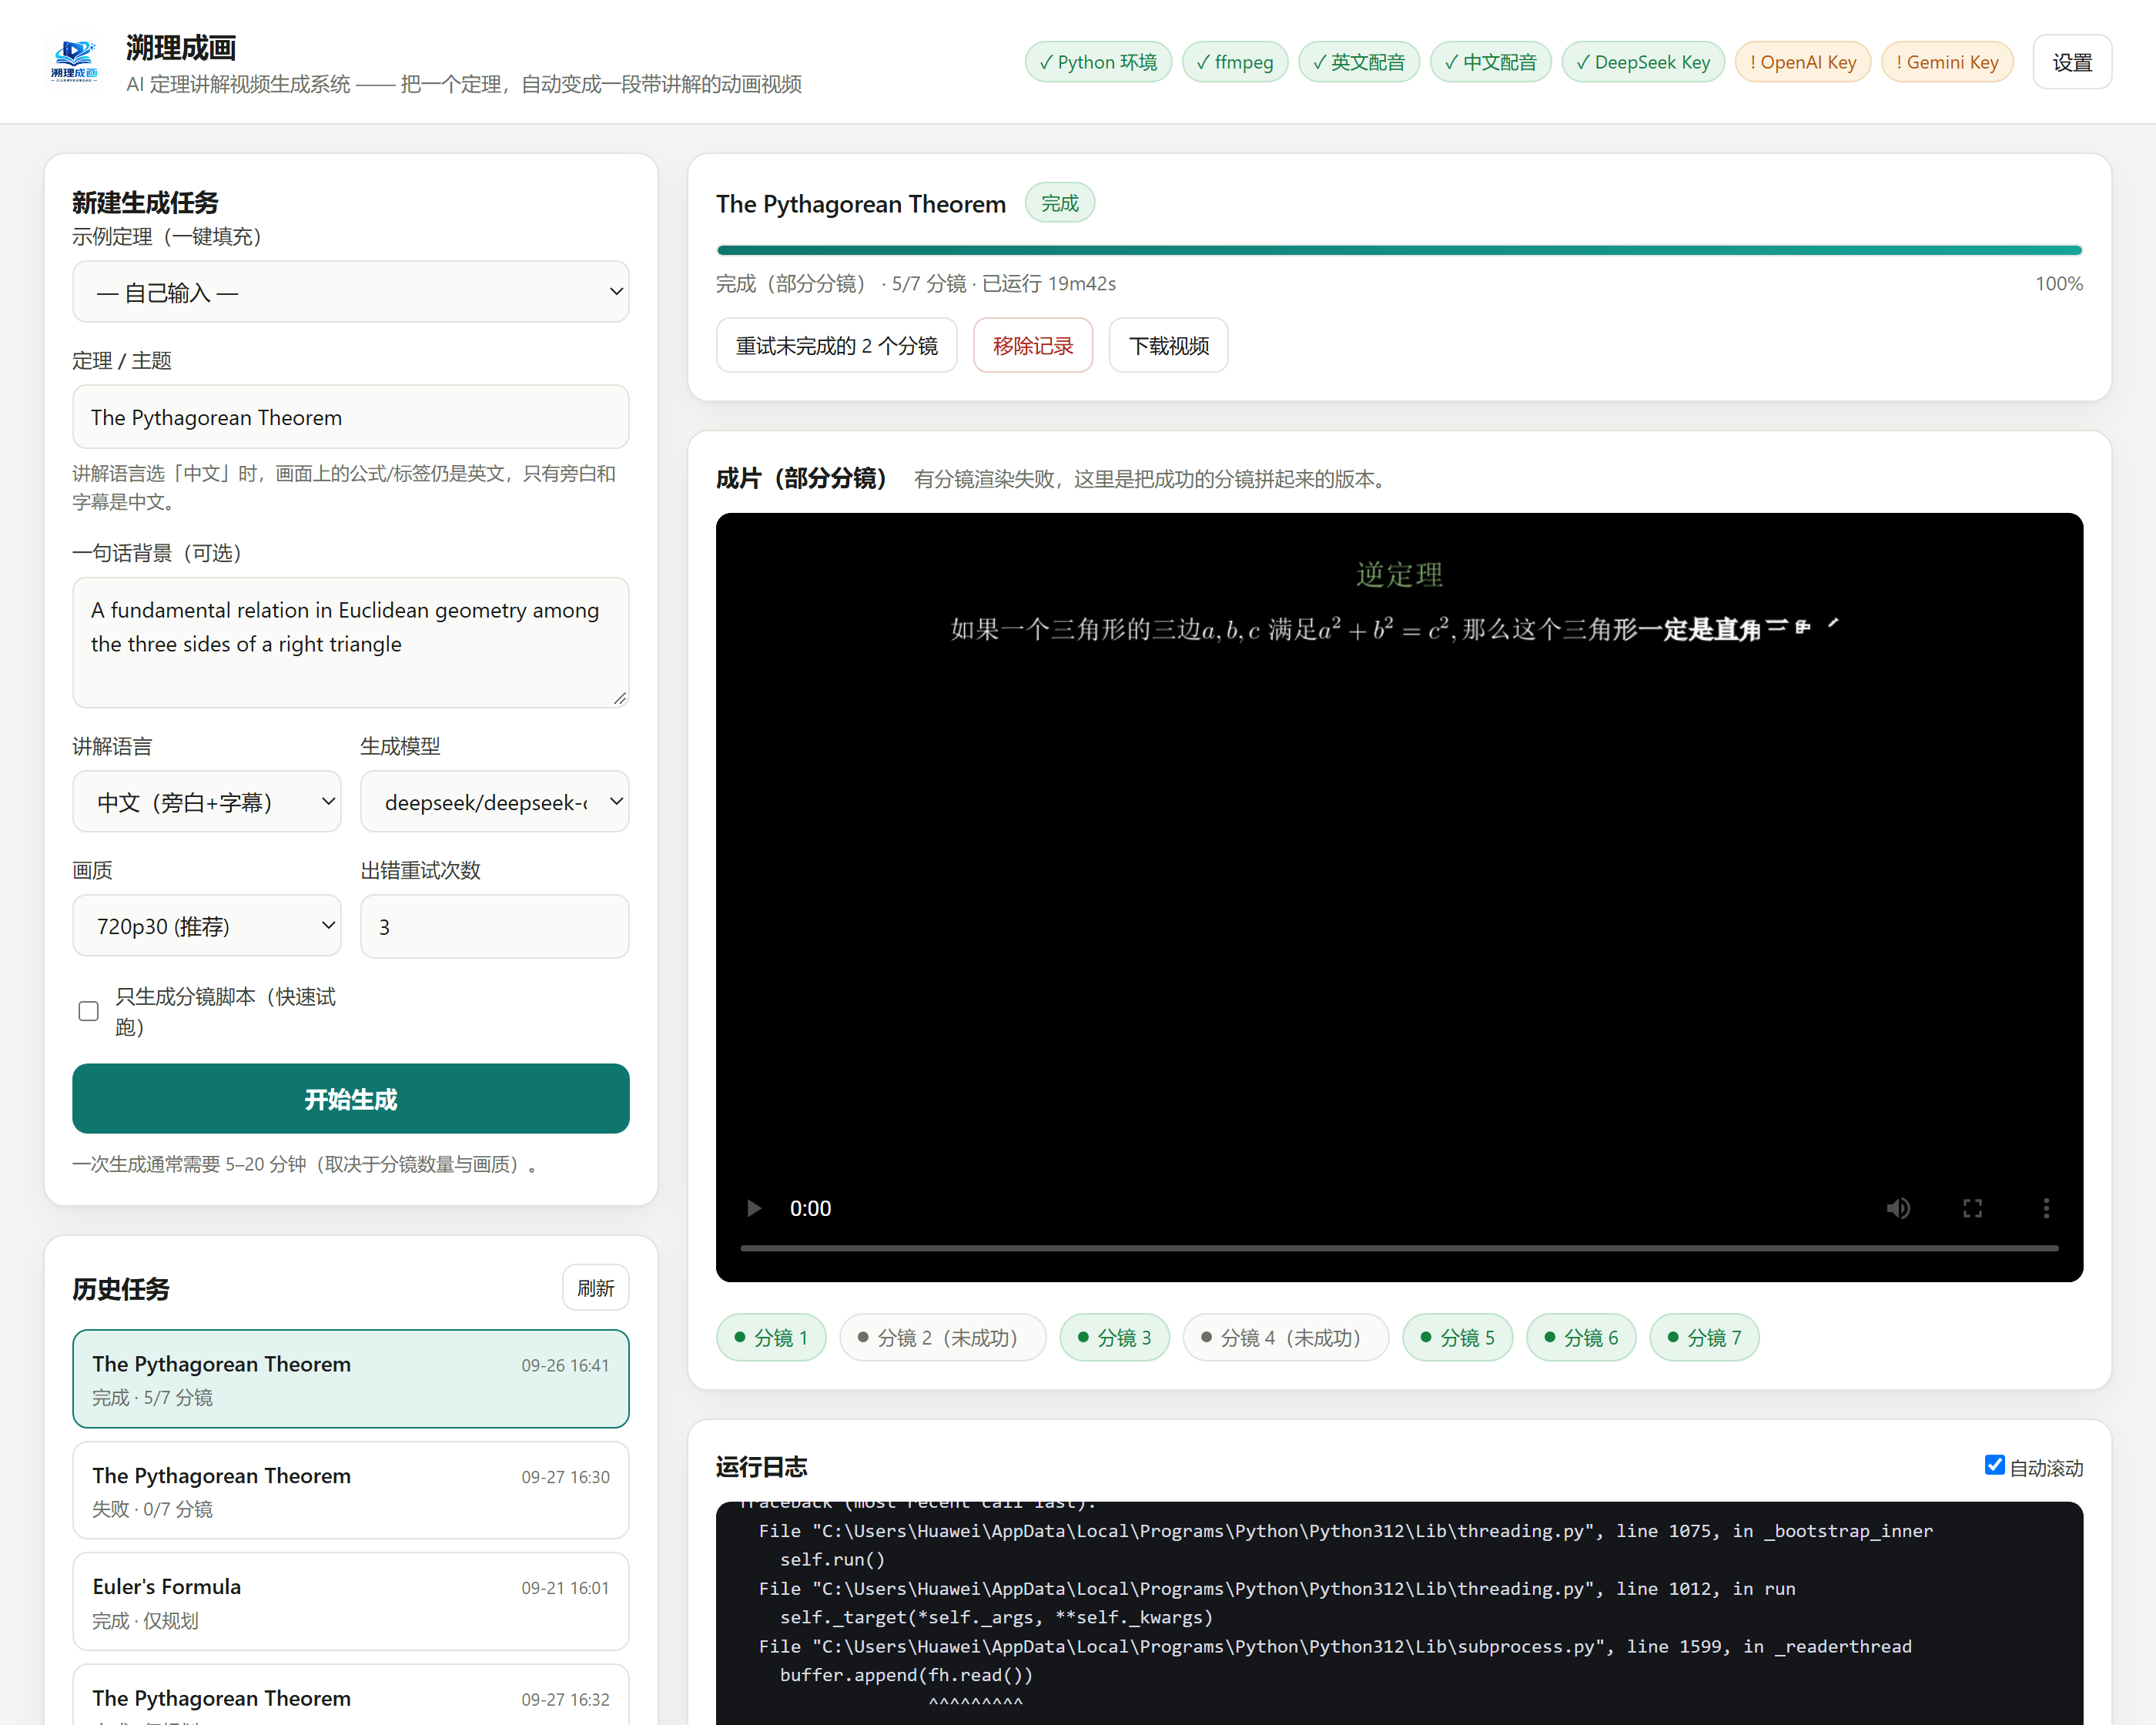
\includegraphics[width=0.99\textwidth]{ui_overview.png}
\caption{系统主界面：左侧为新建任务与历史任务，右侧为任务进度、成片播放、分幕回放与运行日志（播放器画面为实际生成的中文讲解画面帧）}
\end{figure}

\subsection{功能逐条说明}

\subsubsection{一、任务创建与配置}

\textbf{F1 任务创建}：填写定理／主题与一句话背景即可提交，其余参数均有合理默认值；提交后任务进入队列，界面立刻出现该任务并开始刷新状态。\\
\textbf{F2 示例题库}：内置勾股定理、贝叶斯定理、傅里叶级数、微积分基本定理、欧拉公式等已验证主题，选择后自动填充主题与背景说明，用于快速体验与演示。\\
\textbf{F3 环境自检}：界面顶部以状态标签实时显示 Python 环境、ffmpeg、英文配音、中文配音以及三家模型 Key 的可用性；异常项以警示色标出，避免用户提交任务后才发现环境缺件。\\
\textbf{F4 参数配置}：\emph{讲解语言}（中文／英文一键切换）、\emph{生成模型}（可从下拉选择，也可自行添加任意 LiteLLM 格式的模型名）、\emph{画质}（草稿 480p15／推荐 720p30／高清 1080p60）、\emph{出错重试次数}（1--8 次）。\\
\textbf{F5 快速试跑}：勾选「只生成分镜脚本」后跳过渲染阶段，只跑教学法与分镜规划，用几十秒到数分钟验证链路是否通畅、中文旁白是否正常，再决定是否投入完整渲染。

\subsubsection{二、密钥与模型管理}

\textbf{F6 密钥设置}：在设置弹窗中填写 DeepSeek／OpenAI／Gemini 任一密钥，保存后写入本机 \texttt{.env}，不进入代码仓库、不上传任何服务器；留空即表示不修改。\\
\textbf{F7 模型扩展}：可在设置中追加任意模型标识（如 \texttt{openai/gpt-4o}、\texttt{gemini/gemini-2.0-flash-001}），追加后立即出现在模型下拉框中，便于在「效果」与「成本」之间权衡。

\subsubsection{三、过程可观测}

\textbf{F8 实时进度}：显示「分镜总数、已完成分幕数、当前阶段、已运行时长」，并按规划、逐幕生成、渲染、合并四个阶段推进百分比。进度并非估算，而是由产物文件反推，因而与实际进展一致。\\
\textbf{F9 运行日志}：完整输出运行日志并自动滚动，任何一幕失败都能直接看到是哪一幕、报了哪一类错。\\
\textbf{F10 错误人话提示}：把余额不足、额度耗尽、Key 无效、触发限流、上下文超长等接口错误翻译为中文操作建议，直接显示在任务卡片上。\\
\textbf{F11 分幕状态与回放}：以标签形式列出每一幕（完成／未成功），点击已完成的分幕即可单独播放，便于逐幕检查质量或用于教学切片。

\subsubsection{四、结果消费}

\textbf{F12 成片播放与下载}：生成完成后可直接在线播放，也可下载视频文件；成片采用适合网页播放的编码参数，可直接拖拽进度。\\
\textbf{F13 字幕下载}：同时提供中文字幕文件（SRT），可用于二次剪辑、外语翻译或制作双语版本。

\subsubsection{五、容错与恢复}

\textbf{F14 部分成功兜底}：若只有部分分幕渲染成功，系统不会让用户白等——自动把成功的分幕拼接为可播放的「部分分幕」版本，并明确标注，使用户至少拿到可用素材。\\
\textbf{F15 失败分幕重试}：一键重试只重新生成未成功的分幕，已成功的分幕直接复用，避免重复消耗时间与模型额度。\\
\textbf{F16 任务取消与记录管理}：可随时取消运行中的任务；历史记录可移除（仅移除记录，已生成的文件保留在输出目录中）。\\
\textbf{F17 任务持久化}：任务元数据与日志落盘保存，服务重启后仍可查看历史任务的状态与产物路径。

\subsubsection{六、语言与兼容}

\textbf{F18 中英文双语生成}：同一主题可在中文与英文之间切换生成，英文模式与上游行为保持一致；切换语言不需要修改任何代码或配置。\\
\textbf{F19 环境降级策略}：中文语音或 CJK 模板不可用时自动回退（回退英文语音／英文画面），保证流程不中断——\emph{能出片优先于更好看}。\\
\textbf{F20 本地化与隐私}：服务仅监听本机回环地址，密钥、视频、日志全部保留在本机，不向任何第三方上传生成内容。

% ==================== 10 使用说明 ====================
\section{完整使用说明}

\subsection{运行环境与前置条件}

\begin{table}[htbp]
\centering
\small
\caption{运行环境清单}
\begin{tabularx}{\textwidth}{@{}p{3.4cm} p{2.6cm} X@{}}
\toprule
\textbf{项目} & \textbf{是否必须} & \textbf{说明} \\
\midrule
Windows / macOS / Linux & 必须 & 已在 Windows 11 环境完整跑通 \\
Python 3.12 + 项目虚拟环境 & 必须 & 虚拟环境位于项目内，启动脚本自动使用 \\
LaTeX（MiKTeX 等，含 xelatex 与 ctex） & 必须 & 渲染数学公式与中文画面；缺失时中文画面降级为英文 \\
FFmpeg / ffprobe & 必须 & 已随仓库提供于 \texttt{tools/} 目录，无需另行安装 \\
模型 API Key（DeepSeek／OpenAI／Gemini 任一） & 必须 & 在界面「设置」中填写；DeepSeek 成本最低，GPT-4o 类模型成功率更高 \\
网络连接 & 必须 & 调用大模型接口；中文配音使用在线神经语音，需要联网 \\
显卡 & 非必须 & 渲染在 CPU 上完成，显卡仅加速部分可选组件 \\
\bottomrule
\end{tabularx}
\end{table}

\subsection{安装与启动}

\begin{lstlisting}
# 1. 安装依赖（含中文配音 edge-tts）
pip install -r requirements.txt

# 2. 启动 Web 服务（Windows 一键脚本）
powershell -ExecutionPolicy Bypass -File webapp\start.ps1

#    或手动启动
#    $env:PYTHONPATH = (Get-Location)
#    .\.venv\Scripts\python.exe -m uvicorn webapp.app:app --host 127.0.0.1 --port 8765

# 3. 浏览器访问
#    http://127.0.0.1:8765
\end{lstlisting}

端口可通过环境变量调整；默认端口为 8765，以避开常见端口占用。

\subsection{标准操作流程}

\begin{enumerate}
  \item \textbf{启动服务}：执行上述启动脚本，浏览器打开本地地址；
  \item \textbf{检查环境}：查看顶部状态标签，确认 Python 环境、ffmpeg、中英文配音与至少一个模型 Key 为可用状态；
  \item \textbf{配置密钥}（首次使用）：点击右上角「设置」，粘贴至少一个模型 API Key 并保存，状态标签随即变绿；
  \item \textbf{选择主题}：从「示例定理」下拉框一键填充，或自行输入定理名称与一句话背景（建议用英文写数学主题名，讲解语言选择决定旁白与画面语言）；
  \item \textbf{设置参数}：选择讲解语言（默认中文）、生成模型、画质与出错重试次数；
  \item \textbf{快速试跑（建议）}：勾选「只生成分镜脚本」并点击「开始生成」，在 1--6 分钟内确认分镜与中文旁白正常；
  \item \textbf{正式生成}：取消勾选后再次点击「开始生成」，进入完整渲染流程（7 幕、720p 画质约 20 分钟，视模型与画质而定）；
  \item \textbf{观察与干预}：在右侧查看进度与日志；若出现接口额度类错误，按提示处理后可一键重试（已成功的分幕会被跳过）；如需中止可点「取消任务」；
  \item \textbf{获取结果}：生成结束后在线播放成片、下载视频与字幕，或点击分幕标签逐幕回放检查质量。
\end{enumerate}

\subsection{交互指南}

\begin{table}[htbp]
\centering
\small
\caption{界面元素与交互说明}
\begin{tabularx}{\textwidth}{@{}p{3.2cm} p{4.4cm} X@{}}
\toprule
\textbf{界面元素} & \textbf{含义} & \textbf{使用建议} \\
\midrule
顶部状态标签 & 环境与密钥自检结果 & 出现警示项时先处理，再提交任务 \\
示例定理 & 已验证可跑通的主题 & 首次使用与答辩演示优先选择 \\
讲解语言 & 决定旁白、字幕与画面文字语言 & 中文讲解选「中文」；需要英文素材时切换即可 \\
生成模型 & 决定分镜与代码质量 & 追求稳定性用 GPT-4o 类模型；追求低成本用 DeepSeek 并提高重试次数 \\
画质 & 决定分辨率与渲染耗时 & 试跑用 480p15；正式出片用 720p30；1080p60 仅在需要成片交付时使用 \\
出错重试次数 & 单幕自动修复的上限 & 低成本模型建议 3--4 次，高质量模型 1--2 次即可 \\
只生成分镜脚本 & 跳过渲染的快速通道 & 用于验证链路、预览中文旁白与分镜设计 \\
进度条与阶段文字 & 当前所处阶段与已运行时长 & 长时间停留在「渲染分幕」属正常现象 \\
分幕标签 & 每一幕的渲染状态 & 绿色为成功，可点击单独播放；灰白为未成功 \\
运行日志 & 完整过程输出 & 失败时优先在此定位「哪一幕、什么错」 \\
取消 / 重试 / 移除 & 任务生命周期操作 & 重试仅重跑未成功的分幕，已完成的不会重复渲染 \\
下载视频 / 字幕 & 结果导出 & 视频可直接嵌入课件；字幕可用于二次剪辑或多语版本 \\
\bottomrule
\end{tabularx}
\end{table}

\subsection{常见问题自助排查}

\begin{table}[htbp]
\centering
\small
\caption{常见故障与处理方式}
\begin{tabularx}{\textwidth}{@{}p{4.6cm} X@{}}
\toprule
\textbf{现象} & \textbf{原因与处理} \\
\midrule
提交后立刻失败，提示缺少 API Key & 未配置任何模型密钥。打开「设置」填写并保存 \\
提示余额不足／额度耗尽 & 模型账户余额或配额不足。充值或更换其他厂商密钥后重试 \\
提示触发限流 & 请求过于频繁。等待片刻后重试，或降低并发（系统默认串行） \\
某一幕反复失败 & 模型生成的动画代码存在难以修复的问题。可提高重试次数、更换能力更强的模型，或先使用「部分分幕」成片 \\
画面出现英文而非中文 & 运行环境缺少 xelatex／ctex，系统自动降级为英文画面。安装后即可恢复中文画面 \\
没有声音 & 中文配音需要联网；若离线，系统会回退英文语音。检查网络与配音依赖状态标签 \\
渲染耗时远超预期 & 与画质、分幕数量、模型速度直接相关。改用 480p15 草稿档或减少分幕数 \\
服务重启后历史任务显示失败 & 任务在运行中被中断，属预期行为；重试即可复用已成功分幕 \\
\bottomrule
\end{tabularx}
\end{table}

\subsection{命令行进阶用法}

除图形界面外，流水线本身支持直接以命令行方式运行，便于批量生成与自动化集成：

\begin{lstlisting}
python generate_video.py \
  --model "deepseek/deepseek-chat" --helper_model "deepseek/deepseek-chat" \
  --output_dir "output/my_exp" \
  --topic "The Pythagorean Theorem" \
  --context "A fundamental relation in Euclidean geometry" \
  --max_retries 3

# 批量生成（读取题库 JSON）
python generate_video.py --model "openai/o3-mini" \
  --output_dir "output/batch" --theorems_path data/thb_easy/math.json
\end{lstlisting}

\begin{notebox}
\textbf{中文模式提示：}以命令行方式运行时，需同时设置讲解语言环境变量（如 \texttt{TEA\_NARRATION\_LANG=zh}）与渲染画质环境变量（如 \texttt{TEA\_MANIM\_QUALITY=-qm}）；Web 界面会自动完成这两项注入，因此推荐非技术用户优先使用界面。
\end{notebox}

% ==================== 11 实测与验证 ====================
\section{实测结果与效果验证}

\subsection{测试环境与用例}

测试环境为 Windows 11 + Python 3.12 + Manim Community 0.18.1 + MiKTeX（xelatex/ctex）+ 随仓库分发的 FFmpeg，渲染画质为 720p30，生成模型为 \texttt{deepseek/deepseek-chat}（成本最低的一档，用于压力测试容错能力），主讲题为「勾股定理（The Pythagorean Theorem）」，语言为中文。

\begin{table}[htbp]
\centering
\small
\caption{实测记录（数据来自本机真实运行日志与产物统计）}
\begin{tabularx}{\textwidth}{@{}p{1.1cm} p{1.5cm} p{1.2cm} p{1.1cm} p{1.3cm} p{2.6cm} X@{}}
\toprule
\textbf{任务} & \textbf{模式} & \textbf{分幕} & \textbf{成功} & \textbf{耗时} & \textbf{各幕代码版本数（v0 起）} & \textbf{产出} \\
\midrule
A & 中文完整生成 & 7 & 5 & 19 分 42 秒 & 2 / 4 / 3 / 4 / 2 / 1 / 1 & 部分分幕成片，时长 493.8 秒（8 分 14 秒） \\
B & 中文完整生成 & 7 & 0 & 13 分 21 秒 & 4 / 4 / 4 / 4 / 4 / 4 / 4 & 无成片（全部达到重试上限） \\
C & 仅分镜规划 & 7 & --- & 5 分 36 秒 & --- & 分镜脚本与逐幕计划（未渲染） \\
\bottomrule
\end{tabularx}
\end{table}

\subsection{结果一致性核验}

任务 A 中成功渲染的 5 幕时长分别为 119.83 秒、27.30 秒、98.50 秒、121.00 秒、131.03 秒，合计 497.66 秒；兜底合并产出的成片实测时长为 493.8 秒，与「成功分幕拼接」的预期一致，说明\textbf{兜底合并逻辑正确地复用了成功分幕，没有丢失或重复视频段}。作为对照，另一次完整生成的英文成片（7 幕全部成功）时长为 511.1 秒、文件体积 9.1 MB、分辨率 1280$\times$720。

\subsection{中文渲染验证（核心能力的直接证据）}

在中文模式的一次真实渲染中，Manim 生成的 LaTeX 源文件共 57 份，其中 \textbf{40 份带有 CJK 支持宏包 \texttt{ctex}，7 份包含中文字符并被成功编译为矢量图形}。以下为其中一份画面元素的实际源码：

\begin{lstlisting}
\usepackage[UTF8]{ctex}
...
<g id='unique000'>\text{如果一个三角形的三边 } a, b, c \text{ 满足 }
a^2 + b^2 = c^2,</g>
<g id='unique001'>\text{那么这个三角形一定是直角三角形。}</g>
\end{lstlisting}

这段源码同时证明了本作品技术方案的两个要点：\textbf{画面中的中文标题与标签可以正常排版}，而\textbf{数学公式保持语言无关的标准 LaTeX}（$a^2+b^2=c^2$ 未被翻译）。

中文旁白与字幕同样验证通过，以下为实际生成字幕文件中的片段：

\begin{lstlisting}
1
00:00:00,000 --> 00:00:13,004
在前面的内容里，我们已经多次接触到直角三角形。现在，让我们正式
认识一下这位"老朋友"。
2
00:00:13,633 --> 00:00:22,828
请注意左下角这个顶点。这里有一个小小的黄色方块——它不是装饰，
而是一个记号，表示这个角恰好是 90°，也就是我们常说的"直角"。
\end{lstlisting}

\subsection{稳定性验证}

\begin{itemize}
  \item \textbf{自动修复确实生效}：任务 A 中 5 幕最终成功，其中 3 幕需要 2 次以上尝试（含一幕达到 4 次），说明修复闭环能够把「首次生成失败」转化为「最终渲染成功」；
  \item \textbf{失败是可诊断的}：任务 B 的 28 次尝试全部留有独立错误日志，失败原因可逐条追溯，而不是一个笼统的「生成失败」；
  \item \textbf{失败不等于零产出}：任务 A 有 2 幕未成功，系统仍产出可播放的 8 分钟成片，避免用户白等 20 分钟；
  \item \textbf{低成本模型的边界被量化}：任务 B 的结果说明，在最低成本模型上「全幕成功」并非稳定可达。这既是本作品容错机制存在的原因，也是第 13.6 节风险分析中的一条真实依据。
\end{itemize}

\subsection{已知局限与后续验证计划}

我们如实列出当前局限：（1）实测样本量仍然偏小，后续计划在 20--50 个定理上做批量统计，形成「一次通过率、平均重试次数、平均耗时」三项核心指标；（2）不同模型写 Manim 代码的能力差异显著，低成本模型在复杂几何构造上失败率仍偏高；（3）中文画面的字距与行距在极端长句下仍需人工微调；（4）自动视觉审阅依赖多模态模型能力，目前只作为可选增强。

% ==================== 12 应用前景 ====================
\section{应用前景}

\subsection{短期：教师与学生的效率工具}

最直接的价值是把「制作一段精确的数学动画」从以周计的成本降到以分钟计。教师可把它当作备课助手，为每节课快速产出难点动画；学生可把抽象概念转成可反复观看的中文讲解，配合字幕精确定位没听懂的那一步。此阶段的落地门槛最低——一台普通电脑、一个模型密钥即可完整使用。

\subsection{中期：教育内容生产的基础设施}

当生成质量稳定后，系统的定位会从「工具」上升为「内容中台」：题库可批量生成配套讲解动画，教辅机构可批量生产课程动画素材，出版社可为教材配套微课，在线教育平台可按知识点批量补齐可视化内容。此时的核心竞争力是\textbf{流水线的稳定性、批量调度能力与模板化风格控制}，而这三项正好是本作品已经完成工程化建设、并可持续积累的部分。

\subsection{长期：多语言、无障碍与个性化学习}

\begin{itemize}
  \item \textbf{多语言出海}：语言在本作品中被设计为可插拔的配置项。新增一种语言的成本主要是「语音引擎 + 语言指令」，而无需改动生成流水线，天然适合向多语种教学市场复制；
  \item \textbf{无障碍与辅助学习}：字幕文件独立输出，天然适配听障学习者；画面文字与旁白一致，也便于注意力障碍学习者聚焦理解；
  \item \textbf{个性化学习}：同一知识点可生成不同深度版本（直觉版、标准版、严格证明版），配合推送策略形成分层学习路径；
  \item \textbf{教育公平}：在师资薄弱地区，教师可借助系统快速获得标准化动画与讲解，缩小教学资源差距——这与 iCAN 所倡导的创新创业社会价值方向一致。
\end{itemize}

\subsection{技术延展路线}

在现有架构基础上，可沿四条路线继续加深：\textbf{（1）本地化模型}，用开源模型替代云端 API，降低单条成本并提升数据安全；\textbf{（2）模板与风格库}，沉淀学科化的动画模板，减少从零生成的不确定性；\textbf{（3）质量评分闭环}，把上游评测能力前置到生成过程中，自动淘汰低质量分幕并重生成；\textbf{（4）交互式讲解}，在成片基础上支持学习者暂停提问、由模型就地生成补充片段。

% ==================== 13 商业模式 ====================
\section{商业模式}

\subsection{价值主张}

我们出售的不是「视频文件」，而是\textbf{内容产能}：把原本需要多人协作、以周计的数学动画制作，压缩为「一次点击、可预期耗时、可反复重生」的标准动作。对教师而言这是时间；对机构而言这是成本；对学生而言这是理解效率。

\subsection{收入结构}

\begin{table}[htbp]
\centering
\small
\caption{五条收入路径}
\begin{tabularx}{\textwidth}{@{}p{2.8cm} p{5.0cm} X@{}}
\toprule
\textbf{模式} & \textbf{形态} & \textbf{目标客户与定价思路} \\
\midrule
订阅制 SaaS & 免费额度 + 按月／按年订阅，含更高并发、更多模型与更长视频 & 教师与个人创作者；按月付费，价格锚定「一次外包动画制作成本」的极小比例 \\
私有化部署 & 一次性授权 + 年度维护，部署在校内／机构内网，数据不出内网 & 学校、教培机构、企业与出版机构；按坐席或按年授权 \\
B 端定制生产 & 按知识点／课时交付成片与源文件，提供模板风格定制 & 出版社、在线教育平台；按内容量计价 \\
内容分成 & 与创作者合作生产内容，按平台播放收益分成 & 知识类内容创作者；零预付、收益共享 \\
能力输出（API） & 开放「定理 → 讲解视频」接口，供第三方平台集成 & 教育类应用与工具厂商；按调用量计价 \\
\bottomrule
\end{tabularx}
\end{table}

\subsection{成本结构}

主要成本由三部分构成：\textbf{模型调用成本}（与分幕数量、重试次数成正比，是本作品最需要优化的变量）、\textbf{渲染算力成本}（本地渲染时近乎为零，云端批量渲染时为服务器成本）、\textbf{人工成本}（模板维护、质量抽检、客服支持）。值得注意的是，本作品的多项工程改进都直接作用于成本：错误速查表减少无效重试，部分成功兜底减少无效等待，画质档位让「预览」与「交付」使用不同成本。

\subsection{分阶段落地路径}

\begin{enumerate}
  \item \textbf{第一阶段（已完成）}：单机版可用，中文全链路跑通，具备完整的生成、观测与容错能力；
  \item \textbf{第二阶段（近期）}：提升稳定性与批量能力——扩充常见错误清单、引入质量评分与自动重生成、支持批量题库生成与统一风格模板；
  \item \textbf{第三阶段（中期）}：从工具走向服务——云端任务队列、账号与额度体系、内容资产库、团队协作与审核流程。
\end{enumerate}

\subsection{竞争格局}

\begin{table}[htbp]
\centering
\small
\caption{与替代方案的对比}
\begin{tabularx}{\textwidth}{@{}p{2.9cm} p{2.6cm} p{2.4cm} p{2.5cm} X@{}}
\toprule
\textbf{方案} & \textbf{中文讲解} & \textbf{数学精确性} & \textbf{成本／门槛} & \textbf{关键差距} \\
\midrule
人工制作动画 & 可满足 & 高 & 高成本、长周期 & 无法批量，个体教师难以承担 \\
通用 AI 视频工具 & 可满足 & 低（画面为生成式素材，公式与图形不可控） & 低门槛 & 讲不清数学，难以精确呈现推导过程 \\
上游开源引擎（英文） & 不支持 & 高 & 需命令行与英文 & 中文用户无法直接使用，失败即无产出 \\
通用屏幕录制＋口播 & 可满足 & 中（依赖讲解者水平） & 低 & 无动画过程，抽象概念仍难讲清 \\
\textbf{本作品} & \textbf{支持（旁白／字幕／画面）} & \textbf{高（确定性代码渲染）} & \textbf{浏览器一键，成本可控} & \textbf{同时满足中文、精确与低成本三项要求} \\
\bottomrule
\end{tabularx}
\end{table}

\subsection{风险与对策}

\begin{table}[htbp]
\centering
\small
\caption{主要风险与应对}
\begin{tabularx}{\textwidth}{@{}p{2.6cm} p{4.6cm} X@{}}
\toprule
\textbf{风险} & \textbf{具体表现} & \textbf{应对策略} \\
\midrule
开源许可风险 & 上游声明「仅供研究用途，不鼓励商业使用」 & 在作品文档与对外材料中如实标注；商业化前须获得作者许可，或以自研／可商用组件替换引擎核心（详见第 14 章） \\
模型能力依赖 & 低成本模型生成代码失败率偏高（任务 B 即为实证） & 强化错误清单与修复闭环；引入质量评分自动重生成；向用户明确「模型与稳定性」的对应关系 \\
算力与耗时 & 高清渲染耗时长 & 提供画质档位；渲染本地化；后续支持任务排队与夜间批处理 \\
内容准确性 & 大模型可能讲错或表述不严谨 & 保留完整过程与字幕便于人工复核；引入评测与抽检机制；面向教学场景明确定位为「辅助素材」 \\
抄袭质疑 & 复用开源项目易被误解为原创包装 & 全流程标注出处、保留原许可与提交历史、明确区分「上游能力」与「本作品增量」 \\
\bottomrule
\end{tabularx}
\end{table}

% ==================== 14 声明 ====================
\section{合规性与原创性声明}

\subsection{著作权与出处标注}

\begin{enumerate}
  \item 本作品的核心生成引擎来自开源项目 \textbf{TheoremExplainAgent}（ACL 2025 主会 Oral，TIGER-AI-Lab，MIT 协议）。仓库中\textbf{完整保留}其 LICENSE 文件、作者引用信息与原始提交历史，未做任何权属替换；
  \item 本作品的全部增量（中文化改造、稳定性改造、容错机制、Web 服务与界面、中文语音引擎、CJK 排版方案、工具与脚本）均为本次工作新增，均可通过版本差异逐项对照，并在上文第 1.3、7.3 节中明确区分；
  \item 本作品\textbf{不声称}拥有定理讲解视频生成算法的原创性，也不将上游成果署名为己有。
\end{enumerate}

\subsection{关于上游「仅供研究」声明的说明}

上游项目在 README 中附有 research-only 声明，明确不鼓励将其代码库用于商业应用。我们尊重这一声明，并因此明确：

\begin{itemize}
  \item 本作品当前定位为\textbf{参赛与教学研究用途}，第 13 章描述的商业模式属于\textbf{路径规划}，而非当前的商业使用行为；
  \item 若进入商业化阶段，将优先完成以下工作之一：\textbf{（a）}与上游作者沟通并取得授权；\textbf{（b）}将生成引擎替换为自研或采用可商用许可的替代实现，仅保留「中文语音、CJK 排版、容错闭环、Web 服务」等完全属于本作品的模块。
\end{itemize}

\begin{notebox}
我们认为，把这一风险主动写进作品文档而不是回避，比在答辩现场被追问更稳妥。工程落地类赛道的评审关注「能不能真正做出来并持续运行」，而可持续性首先取决于合规性。
\end{notebox}

\subsection{数据与隐私}

系统仅在本机运行并监听回环地址；模型密钥保存在本地 \texttt{.env} 文件且不进入版本库（\texttt{.gitignore} 已排除）；生成的视频、字幕、日志、代码版本全部保留在使用者本机；除必要的模型接口调用外，不向任何第三方上传生成内容。

\subsection{内容责任}

大模型存在出错的可能，系统因此保留完整的过程产物（分镜计划、逐幕代码、错误日志、字幕文本），以便使用者复核与修改。本作品面向教学场景定位为\textbf{辅助素材生成工具}，正式教学使用前建议由使用者做内容审核。

\section*{致谢}
\addcontentsline{toc}{section}{致谢}

感谢 TheoremExplainAgent 原作者团队（TIGER-AI-Lab）开源了优秀的定理讲解视频生成框架，使本次中文化与工程化落地成为可能；感谢 Manim Community、manim-voiceover、LiteLLM、edge-tts、MiKTeX 与 FFmpeg 等开源项目提供了坚实的技术基础。

\appendix
\section{主要文件结构}

\begin{lstlisting}
generate_video.py                 # 生成流水线入口（命令行）
src/core/video_planner.py         # 教学法规划、分镜大纲、逐幕细化
src/core/code_generator.py        # Manim 代码生成 + 错误聚焦与自动修复
src/core/video_renderer.py        # 渲染、配音、字幕、合并（含 CJK 字幕重排）
src/utils/tts_service.py          # 语音服务工厂 + CJK LaTeX 模板自动注入
src/utils/edge_tts_voiceover.py   # 中文神经语音服务
src/utils/kokoro_voiceover.py     # 英文语音服务（上游）
task_generator/                   # 全部提示词（含语言指令与常见错误速查表）
task_generator/prompts_raw/code_common_errors.txt   # 常见错误速查表（本作品新增）
webapp/app.py                     # FastAPI 服务、任务队列、进度与日志接口
webapp/static/                    # 前端页面（原生 HTML/CSS/JS，零构建）
webapp/jobs/                      # 任务元数据与日志
eval_suite/  evaluate.py          # 自动评测脚本（文本/图像/视频）
data/thb_*/                       # 定理评测题库（四学科、三档难度）
tools/ffmpeg.exe, ffprobe.exe     # 随仓库分发的视频处理工具
\end{lstlisting}

\section{关键改动速查（相对上游）}

\begin{table}[htbp]
\centering
\small
\caption{本作品相对上游的主要代码改动}
\begin{tabularx}{\textwidth}{@{}p{4.6cm} X@{}}
\toprule
\textbf{文件／模块} & \textbf{改动内容} \\
\midrule
\texttt{tts\_service.py}（新增） & 语音服务工厂；中文模式下自动注入 CJK LaTeX 模板；环境缺失时静默降级 \\
\texttt{edge\_tts\_voiceover.py}（新增） & 中文神经语音服务，与英文语音服务接口一致 \\
\texttt{task\_generator/} & 新增中文旁白与画面文字的语言指令注入（英文模式下不生效） \\
\texttt{prompts\_raw/} & 新增常见错误速查表；更新代码生成提示词（语音工厂、CJK 模板注意事项） \\
\texttt{code\_generator.py} & 新增错误日志聚焦裁剪；修复提示词注入常见错误清单 \\
\texttt{video\_renderer.py} & 新增 CJK 字幕重排、渲染画质可配置、渲染目录动态解析；修复 ffmpeg 管道死锁 \\
\texttt{generate\_video.py} & 注入常见错误上下文；修复视觉修复分支的未定义变量缺陷 \\
\texttt{allowed\_models.json} & 新增 DeepSeek 系列模型，便于低成本使用 \\
\texttt{requirements.txt} & 新增 \texttt{edge-tts} 依赖 \\
\texttt{webapp/} & 全新：FastAPI 服务、任务队列、进度与日志接口、前端界面 \\
\bottomrule
\end{tabularx}
\end{table}

\end{document}
